\chapter{Dynamic Model} \label{ch:model}


%ADD in this section etc
A mathematical model of the system needs to be derived in order to simulate and study the effects of nonlinear Geometric Control. In Section \ref{sec:mod.geometric} an introduction is given about Geometric Mechanics. This is a modern description of the classical mechanics from the perspective of Differential Geometry, which is a discipline in mathematics that studies manifolds and their geometric properties, using the tools of calculus. 

The assumptions that are applied to simplify the model are shortly discussed in Section \ref{sec:mod.assum}. Next, in Section \ref{sec:mod.QRLmod} a dynamical model of the \a{qr}-Load system is obtained with Geometric Mechanics, resulting in a compact, coordinate-free, unambiguous representation of the dynamics, described on nonlinear manifolds.

\section{Geometric Mechanics}\label{sec:mod.geometric}
To derive the equations of motions, traditional modeling methods often parameterize the rotations in a local coordinate system. 
This can be done with Euler Angles, and despite this parametrization might result in singularities, this is a commonly used method to describe rotations. 
There are 24 possible sets of Euler angles and many different conventions are used, which introduces ambiguity. The definition of Euler angles is not unique and a sequence of rotations is not commutative. Therefore, Euler angles are never expressed in terms of the external frame, or in terms of the co-moving rotated body frame, but in a mixture.

Euler angles are kinematically singular since the transformation from their time rates of change to the angular velocity vector is not globally defined. Furthermore, when angular errors are large, the difference in Euler angles is no longer a good metric to define the orientation error. 
%Local coordinates often require symbolic computational tools due to complexity of multi-body systems. 
Hence, the error is rather written as the required rotation to get from the current to a desired orientation, which can be achieved by considering geometric properties of the system.

In Geometric Mechanics the configuration space of systems is a \textit{group manifold} instead of a Euclidean space. The kinetic and potential energies are expressed in terms of this configuration space and their tangent spaces. It explores the geometric structure of a Lagrangian- or Hamiltonian system through the concepts of vector calculus, linear algebra, differential geometry, and nonlinear control theory. Geometric mechanics provides fundamental insights into the nonlinear system mechanics and yields useful tools for dynamics and control theory.

%As a result, the equations of motion and the control systems can be developed on a configuration manifold in a coordinate-free, compact, unambiguous manner, while singularities of local parameterization are avoided.

%
%

To illustrate different configuration spaces, an example is given of a simple 2-link arm, see Figure \ref{fig:mod.arm}.
The configuration is defined by the angles of rotation $ q_1$ and $ q_2$. Figure \ref{fig:mod.armcartesian} represents the configuration space in a Cartesian coordinate system, where the markers represent identical configurations. This shows that this representation suffers from singularities where multiple points in one representation are being mapped onto a single point in another representation. Figure \ref{fig:mod.armtorus} represents the configuration space as a geometric shape called a \textit{torus}, a smooth manifold where every configuration is mapped uniquely.
\begin{figure}[h!]
	\centering
	\makebox[.3\textwidth][c]{\subfloat[][\label{fig:mod.arm}]{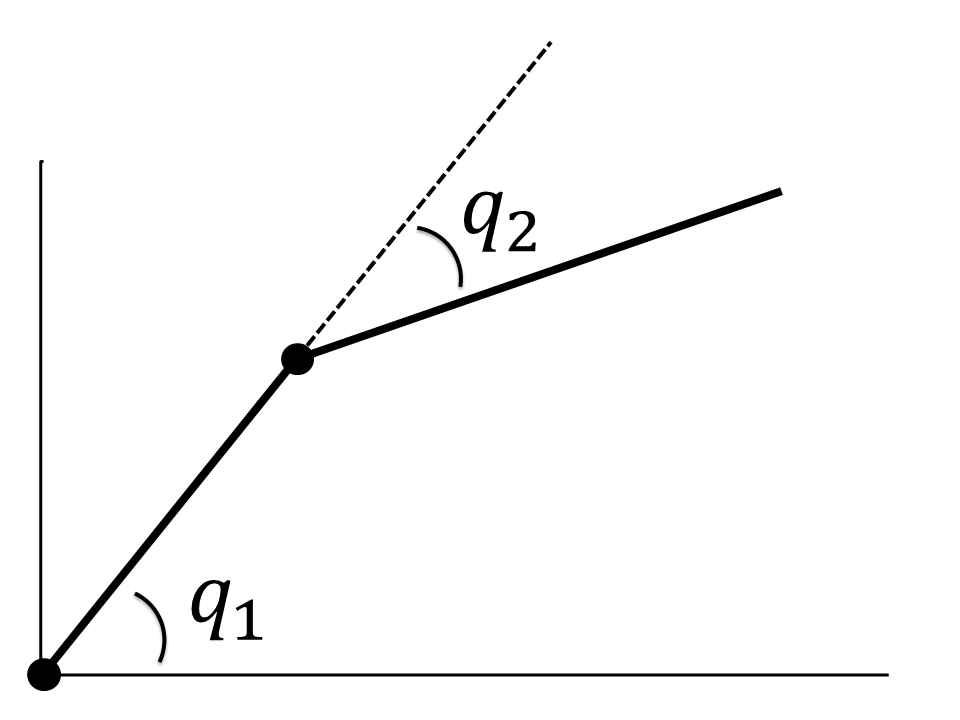
\includegraphics[trim={0 -1cm 0 0},clip,width=.35\textwidth]{./StyleStuff/robotarm.png}}}
	\makebox[.3\textwidth][c]{\subfloat[][\label{fig:mod.armcartesian}]{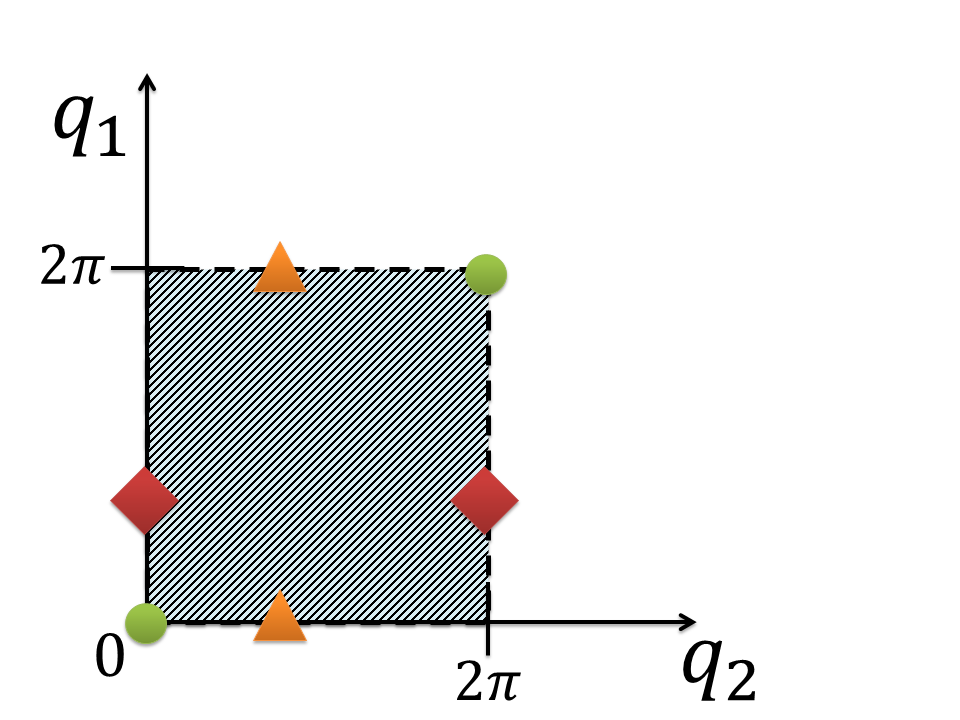
\includegraphics[trim={-3.5cm 0 0 0},clip,width=.45\textwidth]{./StyleStuff/armcartesian.png}}}
	\makebox[.3\textwidth][c]{\subfloat[][\label{fig:mod.armtorus}]{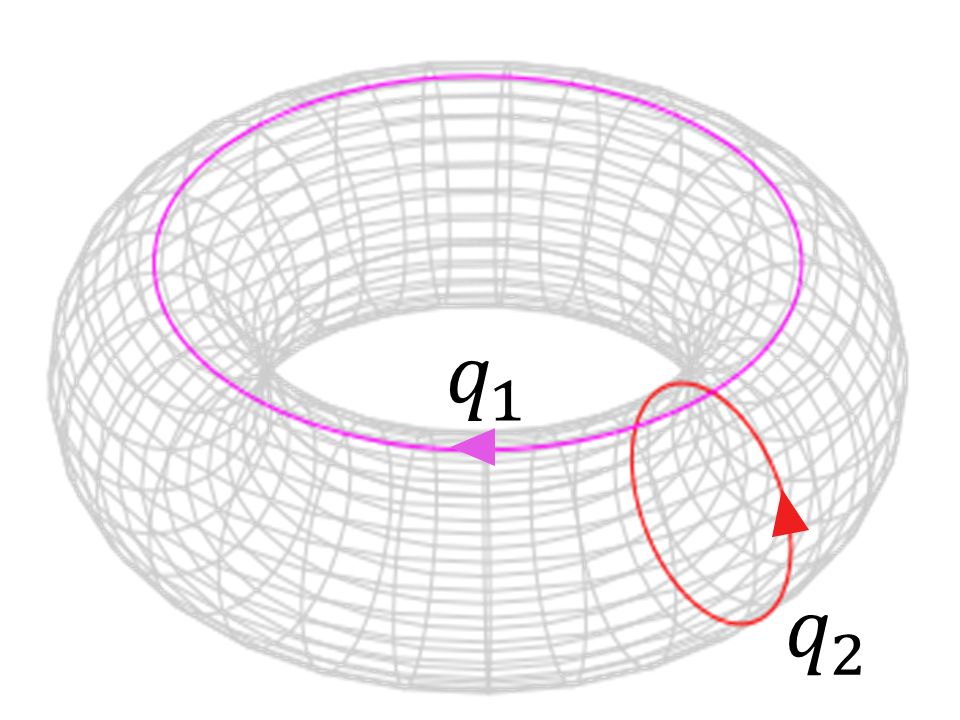
\includegraphics[trim={0 -2cm 0 0},clip,width=.375\textwidth]{./StyleStuff/torus.png}}}
	\caption{Configuration Space of a 2-link arm\label{fig:mod.armmanifold}}
\end{figure}		

%CHECK
%Mechanics studies the dynamics of physical bodies acting under forces and potential fields. 
%In Lagrangian mechanics, the trajectories are obtained by finding the paths that minimize the integral of a Lagrangian over time, called the action integral. 
%Rigid body dynamics are characterized by Lagrangian/Hamiltonian dynamics. The dynamics of a Lagrangian system has unique geometric properties and these are exploited to obtain Euler-Lagrange equations. The resulting intrinsic form of the Euler-Lagrange equations are more compact than equations expressed in terms of local coordinates.

\paragraph{Manifolds}
%ADD  manifolds
The fundamental object of differential geometry a manifold. A manifold is a mathematical space, a collection of points, that locally resembles Euclidean space near each point. Examples are a plane, a ball, a torus and a sphere. Manifolds are important objects in mathematics and physics because they allow more complicated structures to be expressed and understood in terms of the relatively well-understood properties of simpler spaces. In Figure \ref{fig:mod.manifold} is illustrated that each point of an n-dimensional manifold has a neighborhood that is homeomorphic to the n-dimensional Euclidean space, meaning that there is a continuous function describing the relation between these spaces.

\begin{figure}[h!]
	%ADD figure of local space on manifold to cartesian space. Sphere onto R2
	%CHECK \url{https://en.wikipedia.org/wiki/Differentiable_manifold}
	\centering
	\makebox[\textwidth][c]{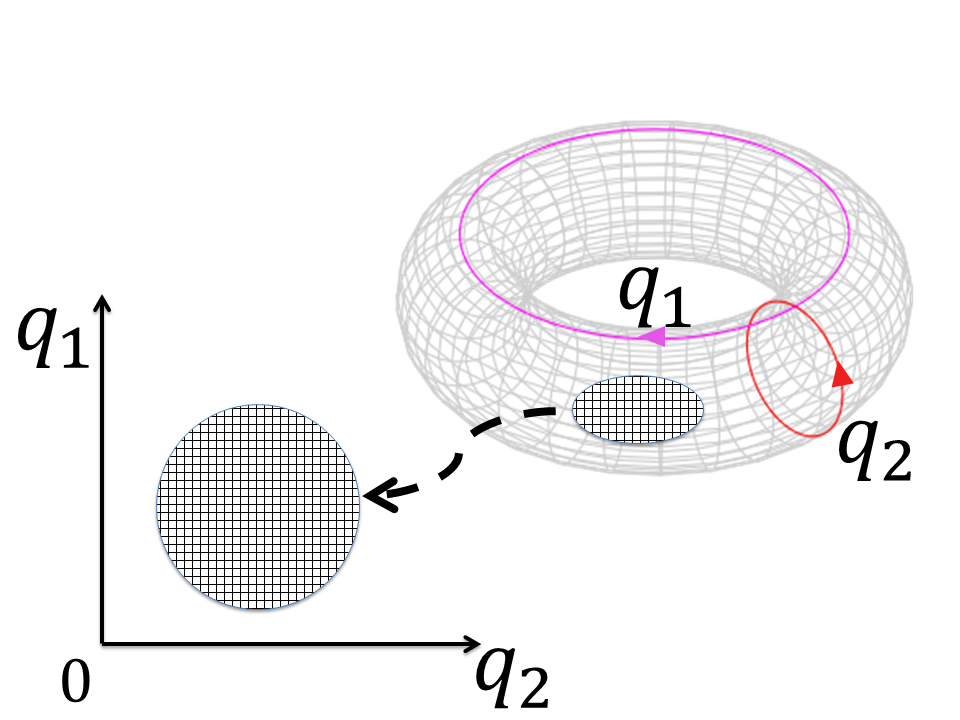
\includegraphics[width=.45\textwidth]{./StyleStuff/manifold.png}}
	\caption{A manifold locally resembles a Euclidean space\label{fig:mod.manifold}}
\end{figure}

%ADD 
%An Introduction to Differentiable Manifolds is given by \cite{Boothby2003}. 

A differentiable manifold is a smooth and continuous manifold and is locally similar enough to a linear space to allow to do calculus. One can define directions, tangent spaces, and differentiable functions on such a manifold. 
Taking the derivative at a point on a manifold is equivalent to a tangent vector at that point. Meaning that derivatives are conceptually equivalent to an infinitesimally short tangent vector. 
Each point of an n-dimensional differentiable manifold has a tangent space, which is an n-dimensional Euclidean space consisting of all the tangent vectors of all curves that pass through that point. 

In Figure \ref{fig:mod.tspace} the manifold $ \mathbb{S}^2 $ is represented as a sphere, with a tangent space at point $ x $, denoted by $ T_x\mathbb{S}^2 $. 
This illustrates the concept of the relation between $ v $, the derivative of $ x $ in Cartesian space, and the tangent space in on the manifold.
\begin{figure}[h!]
	\centering
	%ADD fig sphere with tangent bundle at x
	\makebox[.49\textwidth][c]{\subfloat[][Representation of a manifold with a tangent space \label{fig:mod.tspace}]{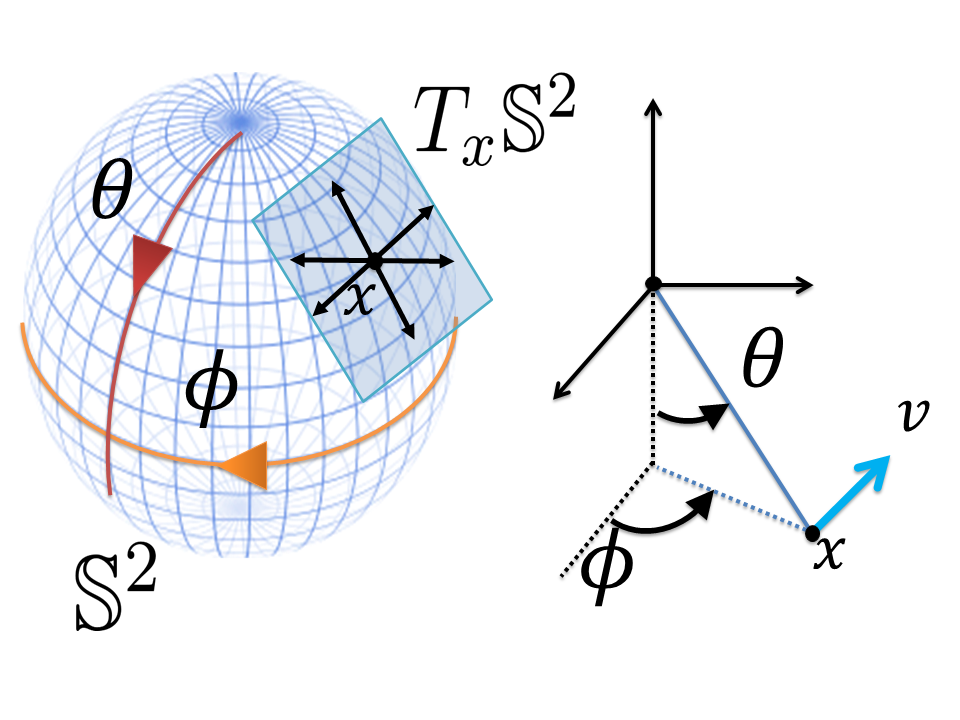
\includegraphics[width=.45\textwidth]{./StyleStuff/tangent.png}}}
	%ADD fig space with SO(3) and so(3)
	\makebox[.49\textwidth][c]{\subfloat[][Identity map of $ SO(3) $ with Lie Algebra $ \mathfrak{so}(3) $ \label{fig:mod.so3}]{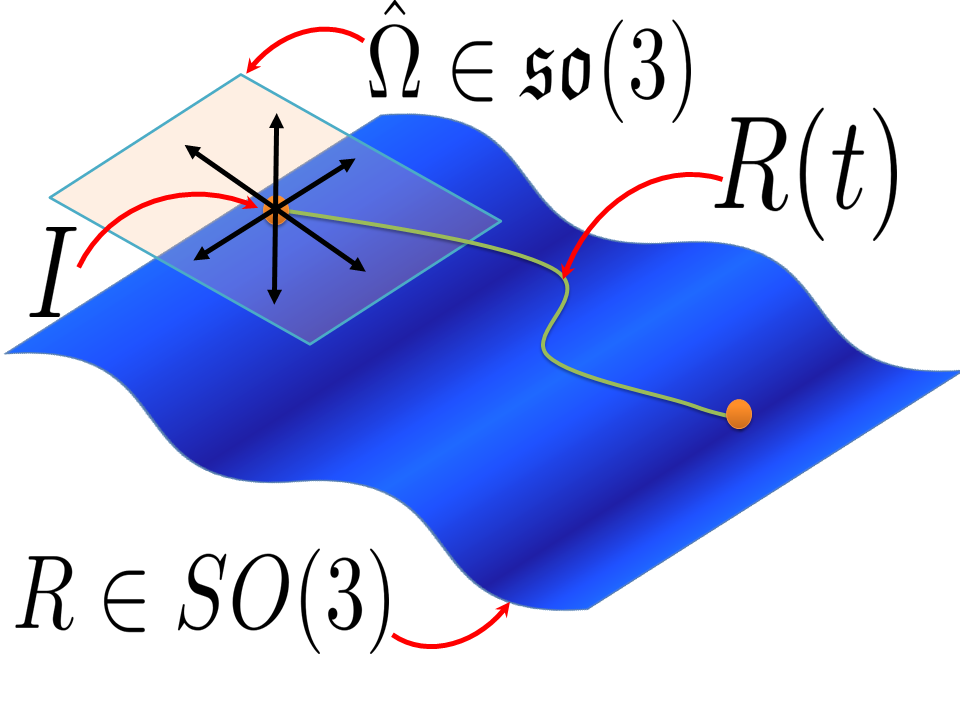
\includegraphics[width=.45\textwidth]{./StyleStuff/so3.png}}}
	\caption{Manifolds and Tangent Spaces\label{fig:}}
\end{figure}		

\subparagraph{Configuration Spaces}
Rotation matrices are used to provide a global representation of the attitude of a rigid body, by mapping a representation of vectors expressed in \BF to a representation expressed in \IF \cite{Chaturvedi2011,Murray1994}. 
The configuration of the \a{qr} attitude is a rotation matrix $ R $ in the Special Orthogonal Group $ SO(3) $ defined as
\begin{equation}\label{eq:SO3}
SO(3) \triangleq \left\lbrace R\in\mathbb{R}^{3\times3}|RR^T=I_{3\times3}, det(R)=1\right\rbrace 
\end{equation}

%CHECK nodig?
%The configuration manifold for combined translational and rotational motion of a rigid body is the special Euclidean group $ SE(3) $, which is a semi-direct product of $ SO(3) $ and $ \mathbb{R}^3 $.

$ SO(3) $ is the group of all rotations about the origin of a 3-D Euclidean space, which preserves the origin, Euclidean distance and orientation.
Several methods exist to describe rotations, such as \textit{Euler Angles}, quaternions or rotation matrices. 
The main disadvantages of Euler angles are that some functions have singularities and they are a less accurate measure for the integration of incremental changes in attitude over time, compared to other methods. 
In Geometric Mechanics the rotations are expressed in rotation matrices to avoid these problems. 

Every rotation has a unique inverse rotation and the identity map satisfies the definition of a rotation. The elements of \textit{Lie Algebra} $ \mathfrak{so}(3) $, a property associated with $ SO(3) $, are the elements of the tangent space of $ SO(3) $ at the identity element, see Figure \ref{fig:mod.so3}. 
These elements define the relation between the rotation $ R $ and its derivative $ \dot{R} $, such that
\begin{equation}\label{eq:Rdot}
\dot{R} = R\hat{\Omega}
\end{equation}
For $ n\in \mathbb{N} $, $ \mathfrak{so}(3) $ is is the vector space of skew-symmetric matrices in $ \mathbb{R}^{n\times n} $ and defined as
\begin{equation}\label{eq:so3}
\mathfrak{so}(n) \triangleq \left\lbrace S\in \mathbb{R}^{n\times n}|S^T=-S\right\rbrace
\end{equation}

The linear map $ \hat{\cdot}:\mathbb{R}^3\rightarrow\mathfrak{so}(3) $ is an isomorphism between $ \mathbb{R}^3 $ and the set of $ 3\times 3 $ skew symmetric matrices. $ \cdot^\vee:\mathfrak{so}(3)\rightarrow\mathbb{R}^3 $ denotes the inverse isomorphism. The mapping between the body angular velocity vector $ \Omega\in\mathbb{R}^3 $ and  $ \hat{\Omega}\in\mathfrak{so}(3) $ can be written as
\begin{equation}\label{eq:mod.hatOmega}
\hat{\Omega}=\begin{bmatrix}
0&-\Omega_3&\Omega_2\\
\Omega_3&0&-\Omega_1\\
-\Omega_2&\Omega_1&0
\end{bmatrix},
\quad
\begin{bmatrix}
0&-\Omega_3&\Omega_2\\
\Omega_3&0&-\Omega_1\\
-\Omega_2&\Omega_1&0
\end{bmatrix}^\vee = \Omega
\end{equation}

The configuration space of the load is represented on a 2-sphere, defined as
\begin{equation}\label{key}
\mathbb{S}^2 \triangleq \left\lbrace q\in\mathbb{R}^{3}|q\cdot q=1\right\rbrace 
\end{equation}
%\begin{equation}\label{key}
%\mathbb{S}^2 \triangleq \left\lbrace (x_1, x_2, x_3)\in\mathbb{R}^{3}| \parallel (x_1, x_2, x_3)\parallel=1\right\rbrace 
%\end{equation}
%ADD sphere - tangent space - perpendicular : angular velocity
\begin{equation}\label{key}
\dot{q} = \omega\times q
\end{equation}
where $ \omega $ is the angular velocity of the suspended load.

\section{Modeling Assumptions}\label{sec:mod.assum} 

%CHECK intermediate frame. nodig?
The \a{qr} model representation is shown in Figure \ref{fig:mod.model}. Three Cartesian coordinate frames are defined:\v{5}
\begin{itemize}
	\setlength\itemsep{.2pt}
	\item The body-fixed reference frame \lsymb{$ \{\mathcal{B}\} $}{Body Frame} (Body Frame)
	\subitem with unit vectors \lsymb{$ \{\mathbf{b}_1,\mathbf{b}_2,\mathbf{b}_3\} $}{Unit vectors along the axes of $ \{\mathcal{B}\} $} along the axes
	\item The ground-fixed reference frame \lsymb{$ \{\mathcal{I} \}$}{Inertial World Frame} (Inertial Frame)
	\subitem with unit vectors \lsymb{$ \{\mathbf{e}_1,\mathbf{e}_2,\mathbf{e}_3\} $}{Unit vectors along the axes of $ \{\mathcal{I}\} $} along the axes								
	\item The intermediary frame \lsymb{$ \{\mathcal{C} \}$}{Intermediary Frame}, ($ \{\mathcal{I} \}$ rotated by the yaw angle $ \psi $) 
	\subitem with unit vectors \lsymb{$ \{\mathbf{c}_1,\mathbf{c}_2,\mathbf{c}_3\} $}{Unit vectors along the axes of $ \{\mathcal{C}\} $} along the axes								
\end{itemize}

\begin{figure}[h!]
	\centering
	\makebox[\textwidth][c]{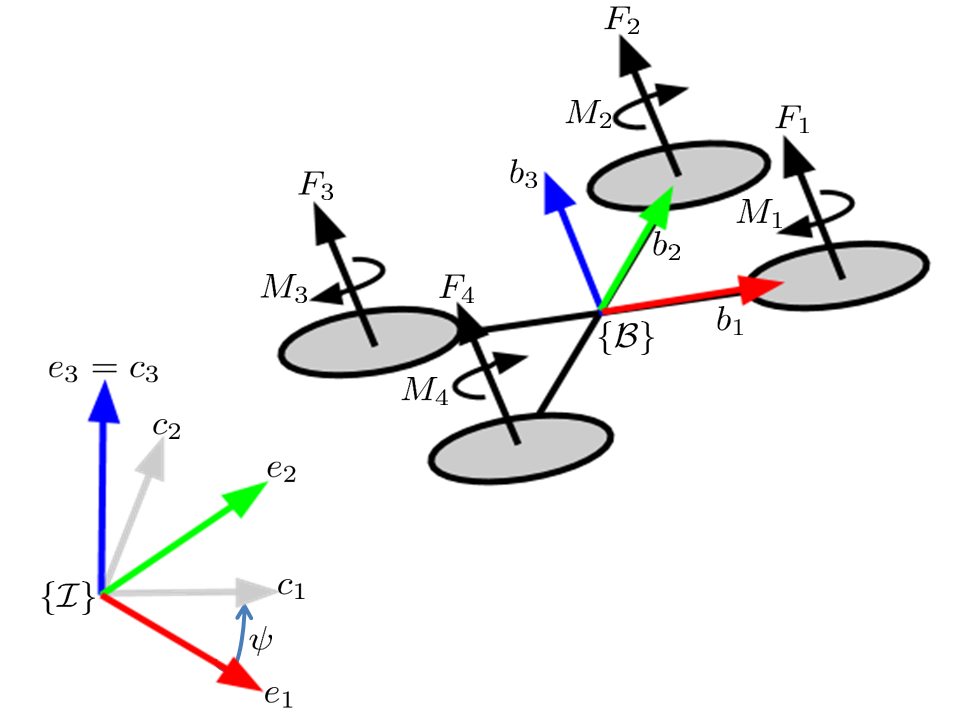
\includegraphics[width=.5\paperwidth]{./StyleStuff/qrmodel.png}}
	\caption{Quadrotor model representation\label{fig:mod.model}}
\end{figure}	



%BART
%***************************************\\
%This is a bit a dead end. I expect something after thsi. FOr example and evaluation of these methods and then the one you are using.
%
%***************************************\\

%CHECK is dit wel nodig?
The complex dynamics of the rotors and their interactions with drag and thrust forces are represented by a simplified model. 
The angular speed \lsymb{$ \omega_i $}{Angular speed of rotor $ i $} of rotor $ i $, for $ i=1,\dots,4 $, generates a force \lsymb{$ F_i $}{Force generated by rotor $ i $} parallel to the direction of the rotor axis of rotor $ i $, given by
\begin{equation}\label{key}
F_i=\left( \frac{K_vK_\tau\sqrt{2\rho A}}{K_t}\omega_i\right)^2=b\omega_i^2 
\end{equation}
where $ K_v,K_t $ are constants related to the motor properties, $ \rho $ is the density of the surrounding air, $ A $ is the area swept out by the rotor, $ K_\tau $ is a constant determined by the blade configuration and parameters, and $ b $ is the thrust factor.\\
The torque around the axis of rotor $ i $, for $ i=1,\dots,4 $, generated due to drag is given by
\begin{equation}\label{key}
M_{i}=\frac{1}{2}R\rho C_DA(\omega_iR)^2=d\omega_i^2
\end{equation}
where $ R $ is the radius of the propeller, $ C_D $ is a dimensionless constant, and $ d $ is the drag constant.

%CHECK directions van de momenten
%CHECK waar is c_tau f gebleven?
For given desired total thrust \lsymb{$ f $}{Total thrust. $ f=\sum_{i=1}^{4}F_i $} and total moment \lsymb{$ M $}{Total moment in \BF. $ M=\begin{bmatrix}	M_\phi&M_\theta&M_\psi	\end{bmatrix}^T $}$=\begin{bmatrix}	M_\phi&M_\theta&M_\psi	\end{bmatrix}^T  $, the required rotor speeds can be calculated by solving the following equation
\begin{equation}\label{eq:omega_i}
\begin{bmatrix}
f\\M_\phi\\M_\theta\\M_\psi
\end{bmatrix}=
\begin{bmatrix}
b&b&b&b\\
0&-lb&0&lb\\
lb&0&-lb&0\\
-d&d&-d&d\\
\end{bmatrix}
\begin{bmatrix}
\omega_1^2\\
\omega_2^2\\
\omega_3^2\\
\omega_4^2\\
\end{bmatrix}
\end{equation}
where \lsymb{$ l $}{Distance from the rotor to the QR CoM} is the distance from the rotor to the \a{qr}'s \a{com} and $ M_\phi, M_\theta, M_\psi $ denote the moments around the $ x, y, z $-axis in \BF, respectively. 

Table \ref{tab:mod.assumptions} shows the most common assumptions that are used for modeling the \a{qr}, simplifying the complexity of the model.

\begin{table}[h!]
	\centering
	\begin{tabular}{|p{\textwidth}|}
		\hline
		\textbf{Modeling assumptions Quadrotor model}\\
		%		\tabitem The rotation of the Earth does not affect the flight of the \a{qr}\\
		\tabitem The structure of the \a{qr} is rigid and symmetric. \\
		\hspace{4mm} Elastic deformations and shock (sudden accelerations) of the \a{qr} are ignored.\\										
		\tabitem The mass distribution of the \a{qr} is symmetrical in the x-y plane.\\
		\tabitem The inertia matrix is time-invariant.\\
		\tabitem Aerodynamic effects acting on the \a{qr} are neglected.\\
		\hspace{4mm} Blade flapping, Turbulence, Ground Effects.\\
		\tabitem The air density around the \a{qr} is constant.\\
		%		\hspace{4mm} An indoor environment guarantees the absence of unpredictable disturbances like wind\\ 
		%		\hspace{4mm} gusts. The model complexity decreases without modeling the effects of wind.\\ 	
		\tabitem The propellers are rigid $ \Rightarrow $ The thrust produced by rotor $ i $ is parallel to the axis of rotor $ i $.\\
		\tabitem Drag factor \lsymb{$ d $ }{Drag factor} and thrust factor \lsymb{$ b $}{Thrust factor} are approximated by a constant.\\
		\hspace{4mm} Thrust force $ F_i $ and moment \lsymb{$ M_{i} $}{Drag moment generated by each propellor} of each propeller is proportional to the square of \\
		\hspace{4mm} the propeller speed. \\
		%		Such that $ F_i = b\omega_i^2$ and $ M_{i} = d\omega_i^2$, where \lsymb{$ \omega_i $}{Angular velocity of rotor $ i $ around its axis, $ i=\{1,2,3,4\} $} is the rotor speed.\\
		\hline
		\textbf{Modeling assumptions Quadrotor-Load model}\\
		\tabitem The cable is modeled as a rigid and massless cable. \\
		\tabitem The cable is connected to a friction-less joint at the origin of the body-fixed. \\
		\tabitem The tension in the cable is considered to be non-zero.\\
		\hspace{4mm} This implies that the QR-Load subsystem, consisting of a separate \a{qr} and Load\\
		\hspace{4mm} in free fall, is disregarded.\\		 
		\tabitem Aerodynamic effects acting on the load are neglected.\\
		\hspace{4mm} reference frame.\\
		%		\tabitem Assumption \\
		%		\hspace{4mm} Details Assumption 2\\
		\hline
	\end{tabular}
	\caption{Modeling assumptions}
	\label{tab:mod.assumptions}
\end{table}

%\begin{table}[h!]
%	\centering
%	\begin{tabular}{|p{\textwidth}|}
%		\hline
%		\tabitem The cable is modeled as a rigid and massless cable. \\
%		\tabitem The cable is connected to a friction-less joint at the origin of the body-fixed. \\
%		\tabitem The tension in the cable is considered to be non-zero.\\
%		\hspace{4mm} This implies that the QR-Load subsystem, consisting of a separate \a{qr} and Load\\
%		\hspace{4mm} in free fall, is disregarded.\\		 
%		\tabitem Aerodynamic effects acting on the load are neglected.\\
%		\hspace{4mm} reference frame.\\
%		\tabitem Assumption \\
%		\hspace{4mm} Details Assumption 2\\
%		\hline
%	\end{tabular}
%	\caption{Modeling assumptions Quadrotor-Load model}
%	\label{tab:mod.assumptionsQRL}
%\end{table}


\section{Quadrotor-Load Model}	\label{sec:mod.QRLmod}
The Quadrotor-Load model is shown in Figure \ref{fig:mod.modelQRL}, where the unit vector \lsymb{$ q$}{Unit vector from \a{qr} to Load} gives the direction from the \a{qr} to the Load expressed in \BF. The focus lies on the subsystem where the cable tension is considered to be non-zero. The position of the \a{qr} and Load are related by
\begin{equation}\label{eq:mod.xQ2xL}
x_Q=x_L-Lq
\end{equation}
where \lsymb{$ x_Q $}{Position of the  of the \a{qr} CoM} is the position of the \a{qr}'s \a{com}, \lsymb{$ x_L $}{Position of the load} is the position of the load, and \lsymb{$ L $}{Length of the cable} is the length of the cable.
\begin{figure}[h!]
	\centering
	\makebox[\textwidth][c]{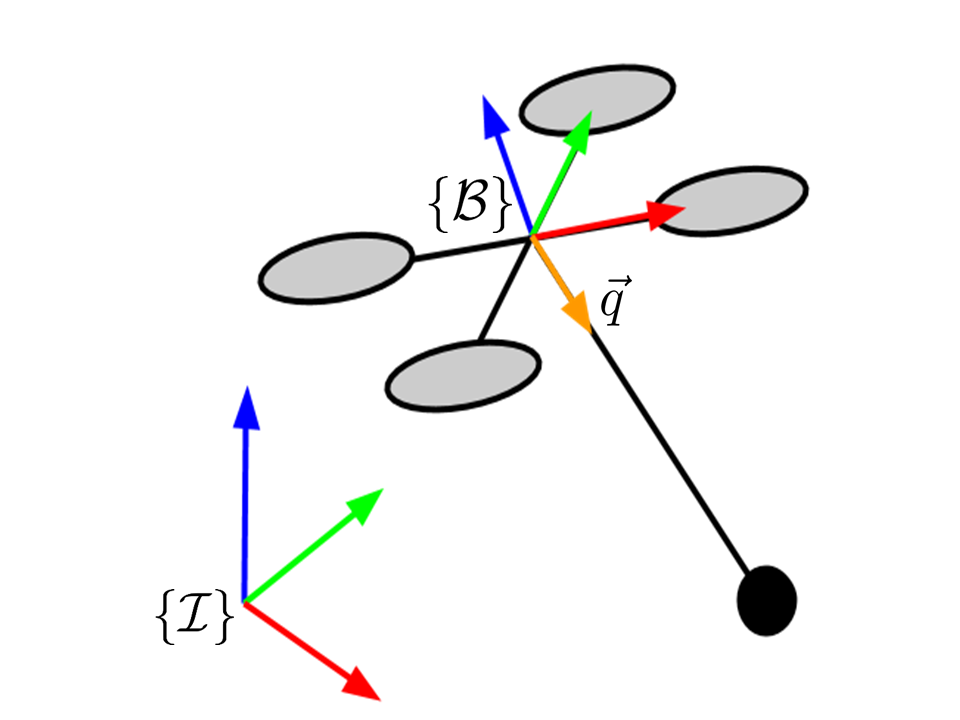
\includegraphics[width=.5\paperwidth]{./StyleStuff/qrlmodel.png}}
	\caption{Quadrotor with Load model representation\label{fig:mod.modelQRL}}
\end{figure}	

Considering the properties of the system, the \a{qr} is described as a rigid body with six degrees of freedom, driven by forces and moments. 
Dynamics and optimal control problems for rigid bodies are studied in \cite{Lee2008}, incorporating their geometric features. The focus lies on obtaining geometric properties of the dynamics of rigid bodies, how their configuration can be described and how these geometric properties are utilized in control system analysis and design. 

%Which means that the motion of a rigid body can be described by a translation of the \acf{com} and a rotation about the \a{com}. 
%The position of \BF is described by a vector evolving on $ \mathbb{R}^3 $, and is represented with respect to \IF.  

The configuration of the \a{qr} can be described by the location of the \a{qr}s \a{com} $x_Q\in \mathbb{R}^3 $, described in the Euclidean space in \IF and by the orientation of \BF, also called attitude, with respect to \IF evolving on a nonlinear space $R\in SO(3) $.\\
The configuration of the load can be described by its location $x_L\in \mathbb{R}^3 $, evolving in Euclidean space, and attitude $ q\in \mathbb{S}^2 $ evolving on a \textit{two-sphere}.\\
%In order to avoid these complexities, 
This results that the dynamics of the \a{qr}-Load system can be globally expressed on the Special Orthogonal Group $SO(3)$, \textit{two-sphere} $ \mathbb{S}^2 $ and Special Euclidean Group $ SE(3) $. This leads to a compact notation of the equations of motion, making the large amount of trigonometric functions unnecessary, that Euler angles normally introduce. 

%LOAD ATTITUDE DYNAMICS
To develop the Euler-Lagrange equations for mechanical systems that evolve on manifolds, an approach developed by \cite{Lee2008,Lee2005,Lee2009,Lee2011} is applied. 

%ADD Hamilton's principle uitleg?
The basic idea is the variations of the curves that are e	

This approach is based on Hamilton's principle, which states that the evolution of a physical system is a solution of the functional equation given by
\begin{equation}\label{key}
\frac{\delta S}{\delta \mathbf{q}(t)}=0
\end{equation}
%CHECK fact, is that what q defines?
where $ \mathbf{q} $ defines the configuration space. $ S $ is the action integral, defined as
\begin{equation}\label{eq:actionintegral}
S=\int_{t_1}^{t_2}\mathcal{L}dt
\end{equation}
where $\mathcal{L}=\mathcal{T}-\mathcal{U} $ is the Lagrangian of the system, and $\mathcal{T},\mathcal{U}$ are the kinetic and potential energy, respectively. 

%Hamilton's principle requires that the first-order change of  $ \delta S $ is zero for all possible perturbations, meaning that the true path is a stationary point of the action integral, which is defined as
Hamilton's principle of least action states that the path a conservative mechanical system takes between two configurations $ q_1 $ and $ q_2 $ at time $ t_1 $ and $ t_2 $, is the one for which Equation \ref{eq:actionintegral} is a stationary point, resulting in
\begin{equation}\label{eq:HamPr}
\delta S=\int_{t_1}^{t_2}\delta\mathcal{L}dt=0
\end{equation}
where $ \delta\mathcal{L} $ is the variation of the Lagrangian. For systems with non-conservative forces and moments, Equation \ref{eq:HamPr} is extended to
\begin{equation}\label{eq:HamPrNon}
\delta S=\int_{t_1}^{t_2}(\delta W+\delta\mathcal{L})dt=0
\end{equation}
where $ \delta W $ is the virtual work. Equation \ref{eq:HamPrNon} is applied to the QR-Load system, where the configuration manifold is $ \mathbb{R}^3\times \mathbb{S}^2\times SO(3) $. With the following states
\begin{equation}\label{eq:mod.S}
\textbf{x}= \begin{bmatrix}x_L& \dot{x}_L& q& \omega&R&\Omega
\end{bmatrix}^T
\end{equation}


\paragraph{Euler-Lagrange} Equation \ref{eq:HamPr} can be satisfied if the following Euler-Lagrange equation holds
\begin{equation}\label{key}
\frac{\delta \mathcal{L}}{\delta \mathbf{q}}-\frac{d}{dt}\frac{\delta \mathcal{L}}{\delta \dot{\mathbf{q}}}=0
\end{equation}
where the Lagrangian $ \mathcal{L}=\mathcal{T}-\mathcal{U} $.
The kinetic energy for the system is denoted as
\begin{equation}\label{key}
\mathcal{T}=\frac{1}{2}m_Q\dot{x}_Q\cdot\dot{x}_Q+\frac{1}{2}m_L\dot{x}_L\cdot\dot{x}_L+\frac{1}{2}\Omega \cdot J\cdot\Omega
\end{equation}
and the potential energy is denoted as
\begin{equation}\label{key}
\mathcal{U}=m_Qgx_Q\cdot e_3+m_Lgx_L\cdot e_3
\end{equation}
where \lsymb{$ g $}{Gravitation constant} is the gravity constant.
The energy can be rewritten in terms of $ q $ and $ x_L $, by substituting Equation \ref{eq:mod.xQ2xL}, giving
\begin{align}\label{key}
\mathcal{T}&=\frac{1}{2}(m_Q+m_L)\dot{x}_L\cdot\dot{x}_L -m_QL\dot{x}_L\cdot\dot{q} + \frac{1}{2}m_QL^2\dot{q}\cdot\dot{q}+\frac{1}{2}\Omega \cdot J\cdot\Omega\\
\mathcal{U}&=(m_Q+m_L)gx_L\cdot e_3-m_QgLq\cdot e_3
\end{align}
The variations of the $ \mathcal{T} $ and $ \mathcal{U} $ are approximated by a first-order Taylor approximation, which results in
\begin{equation}\label{eq:mod.T}
%ADD
\begin{aligned}
\delta\mathcal{T}&\approx \frac{\partial \mathcal{T}}{\partial\dot{x}_L} \delta\dot{x}_L +\frac{\partial \mathcal{T}}{\partial\dot{q}}\delta\dot{q}+\frac{\partial \mathcal{T}}{\partial\Omega}\delta\Omega\\
&=((m_Q+m_L)\dot{x}_L-m_QL\dot{q})\cdot\delta\dot{x}_L+(-m_QL\dot{x}_L+m_QL^2\dot{q})\cdot\delta\dot{q}+J\Omega\cdot\delta\Omega
\end{aligned}
\end{equation}
%Substituting the constraint in Equation \ref{eq:mod.xQ2xL} and its derivative into Equation \ref{eq:mod.T} results in
%\begin{equation}\label{eq:mod.T2}
%%ADD
%\delta\mathcal{T}=
%\end{equation}

\begin{equation}\label{key}
\begin{aligned}
\delta\mathcal{U}&\approx \frac{\partial \mathcal{U}}{\partial{x}_L} \delta{x}_L +\frac{\partial \mathcal{U}}{\partial{q}}\delta{q}\\
&=(m_Q+m_L)ge_3\cdot\delta x_L-m_QgLe_3\cdot\delta q
\end{aligned}
\end{equation}

The first term of virtual work is obtained from $ f $ acting on the \a{qr} and is given by the following term,
\begin{equation}\label{key}
%ADD
\begin{aligned}
\delta W_1&=fRe_3\cdot \sum_{j=1}^{3}\frac{\partial x_Q}{\partial \mathbf{q}_j}\delta \mathbf{q}_j\\
&=fRe_3\cdot(\delta x_L-L\delta q)
\end{aligned}
\end{equation}
where $ \mathbf{q_j}={x_L,q,R} $ and $ x_Q $ is substituted by Equation \ref{eq:mod.xQ2xL}
The second term of virtual work is obtained from $ M $ acting on the \a{qr}. This gives the following term
\begin{equation}\label{key}
\begin{aligned}
\delta W_2&=M\cdot \sum_{j=1}^{3}\frac{\partial\Omega}{\partial \mathbf{\dot{q}}_j}\delta \mathbf{\dot{q}}_j\\
&=M\cdot(R^T\delta R)
\end{aligned}\end{equation}

The variations in energy and the virtual work can be substituted into Equation \ref{eq:mod.S}.

%ADD explain / described in Bullo
Equation \ref{eq:Sfinal} is a function of variations on manifolds, where $ \delta R $ is a variation on $ SO(3) $ and $ \delta q $ is a variation on $ \mathbb{S}^2 $. 
The so called infinitesimal variations required to solve this equation are described as \cite{Bullo2005,Sreenath2013c}
\begin{equation}\label{key}
\begin{aligned}
\delta q&=\xi\times q \in T_q\mathbb{S}^2\text{, where }\xi\in\mathbb{R}^3,\xi\cdot q=0\\
\delta \dot{q}&=\\
\delta R&=R\hat{\eta}\in T_RSO(3)\text{, where } \eta\in\mathbb{R}^3,\hat{\eta}\in\mathfrak{so}(3)\\
\delta \dot{R}&=\\
\delta \hat{\Omega}&=\\
\end{aligned}
\end{equation}

Substituting the variations in energy and the variations in 
\begin{equation}\label{eq:Sfinal}
%ADD
\begin{aligned}
\delta S &= \int_{t_1}^{t_2}(\delta W_1+\delta W_2+\delta\mathcal{T}-\delta\mathcal{U})dt\\
&=\\
&=
\end{aligned}
\end{equation}



%CHECK nodig?
%***************************************\\
%Rigid Body Attitude Dynamics evolve on $ SE(3) $.
%\begin{align}\label{eq:eomrigidbody}
%%CHECK waar komt deze equation vandaan?
%J\dot{\Omega}+\Omega\times J\Omega &= mg\rho\times R^Te_3+u\\ 
%\dot{R} &= R\hat{\Omega}
%\end{align}
%***************************************\\

%CHECK standard newton euler
%***************************************\\
%The equations of motion for a rigid body with configuration $ SE(3) $ are given by the \textit{Newton-Euler equations} \cite{Murray1994}:
%\begin{equation}\label{key}
%\begin{bmatrix}
%	mI&0\\
%	0&\mathcal{I}
%\end{bmatrix}
%\begin{bmatrix}
%	\dot{v}^b\\
%	\dot{\omega}^b
%\end{bmatrix}+
%\begin{bmatrix}
%	\omega^b\times mv^b\\
%	\omega^b\times\mathcal{I}\omega^b
%\end{bmatrix}=F^b
%\end{equation}
%where $ m $ is the mass of the body, $ \mathcal{I} $ is the inertia tensor, and $ V^b=(v^b,\omega^b) $ and $ F^b $ represent the instantaneous body velocity and applied body wrench.
%***************************************\\

%ADD equations of motion
%ADD From .... follows
The \a{qr} attitude kinematics equation is given by
\begin{equation}\label{key}
\begin{aligned}
\dot{x}_L&=\\
(m_Q+m_L)(\dot{v}_L+ge_3)&=\\
\dot{q}&=\\
m_QL\dot{\omega}&=\\
\dot{R}&=R\hat{\Omega}\\
J\dot{\Omega}+\Omega\times J\Omega&=
\end{aligned}
\end{equation}
%\begin{equation}\label{key}
%\hat{\Omega}=\begin{bmatrix}
%0&-\Omega_3&\Omega_2\\
%\Omega_3&0&-\Omega_1\\
%-\Omega_2&\Omega_1&0
%\end{bmatrix}
%\end{equation}



\section*{Summary}

Geometric Mechanics modeling approach is applied to represent the dynamics of the system onto nonlinear configuration manifolds\\

Pro/Cons of Classical Modeling Techniques vs Geometric Modeling\\
Compact, unambiguous, globally defined, \\

In the next chapter nonlinear geometric control is discussed, which is based on the obtained nonlinear geometric representation of the model. 
